\documentclass[12pt]{article}
\usepackage[margin=1in]{geometry}
\usepackage{setspace}
\usepackage{parskip}
\usepackage{graphicx} % Required for inserting images
\usepackage{fullpage}
\usepackage{algorithm}
\usepackage{algpseudocode}
\usepackage{amssymb}
\usepackage{listings}
\usepackage{amsmath}
\usepackage{xcolor}
\usepackage{array}
\usepackage{booktabs}
\usepackage{geometry}
\usepackage{longtable}
\usepackage{url}
\usepackage{pgfplots}
\pgfplotsset{width=10cm,compat=1.9} % ensure backward compatibility

% Define a custom style for R code
\lstdefinestyle{Rstyle}{
    language=R,
    backgroundcolor=\color{cadetblue!10},  % Light cadet blue background
    basicstyle=\ttfamily\footnotesize,  % Font size
    keywordstyle=\color{cadetblue}\bfseries,  % Blue keywords
    commentstyle=\color{darkgreen},  % Green comments
    stringstyle=\color{red},  % Red strings
    identifierstyle=\color{black},  % Black identifiers
    numbers=left,  % Line numbers
    numberstyle=\tiny\color{gray},  % Line number style
    stepnumber=1,
    numbersep=5pt,
    frame=single,  % Frame around the code
    rulecolor=\color{cadetblue},  % Frame color (same as the main theme)
    breaklines=true,  % Break lines if they're too long
    xleftmargin=15pt,  % Left margin for the code block
    xrightmargin=15pt,  % Right margin
    linewidth=\textwidth,  % Ensure the code block fits the page width
    showstringspaces=false,  % Don't highlight spaces in strings
    escapeinside={(*@}{@*)},  % Allow LaTeX commands inside code
}

% Customize the document's appearance
\definecolor{cadetblue}{rgb}{0.372, 0.620, 0.627}  % Define cadet blue color
\definecolor{darkgreen}{rgb}{0.0, 0.39, 0.0}  % Dark Green RGB values

\begin{document}

\title{\textbf{Mind Over Mutation: Exploring Single Nucleotide Polymorphisms Linked to Anxiety \vspace{0.1cm}\\
\large A Genome-Wide Association Study of Anxiety Disorder Risk Loci}}
\author{Emma Shockley}
\date{13 May 2025}
\maketitle

\begin{abstract}
Anxiety disorders are a major public health concern affecting a large proportion of the world's population. This paper reviews the genetic epidemiology of anxiety disorders using Genome-Wide Association Study (GWAS) data and proposes four novel statistical methodologies aimed at correcting for multiple hypotheses. These methods include Bonferroni, Holms, Benjamini-Hochberg, and Benjamini Yekutieli, respectively, to identify novel genes that may also be implicated in anxiety disorders. We present summary statistics, Manhattan plots, and cross-method comparisons across six assessments with varying thresholds, ultimately culminating in the identification of the most significant single nucleotide polymorphisms (SNPs) linked to anxiety disorders while accounting for the complex statistical nuances that demand our attention at this scale. These findings underscore a genetic foundation for anxiety disorders and suggest that continued investigation into candidate genes and biological pathways may enhance our ability to predict the onset of anxiety disorders and inform pharmacogenetic approaches to treatment. We hope this work not only strengthens the foundations of computational neuroscience but also brings us one step closer to individualized mental health solutions.
\end{abstract}
\newpage

\tableofcontents
\newpage

\section{Introduction}
\subsection{Anxiety Disorders}
Anxiety disorders as classified by the Diagnostic and Statistical Manual of Medical Disorders Fifth Edition (DSM-5-TR) span a wide range of illnesses, with the most common being Generalized Anxiety Disorder (GAD). The classification of anxiety manifests not as a homogeneous disorder but rather as a variety of subdisorders including panic disorder, specific phobias, and more. Despite their differing clinical classifications, evidence suggests a common genetic architecture and etiology among conditions, including the core emotions implicated, comorbidity, psychotherapeutic approaches (often selective-serotonin reuptake inhibitors (SSRIs) or selective-norepinephrine reuptake inhibitors (SNRIs)), pathophysiological mechanisms, and genetic overlap \cite{Li2024}. This paper will synthesize genetic findings across various anxiety disorders to assess the complex genetic architecture underlying the entire spectrum of anxiety-related conditions. \par

While anxiety as a physiological response is an evolutionarily beneficial adaptive human characteristic, GAD is characterized by excessive fear, worry, and overwhelm, causing significant distress and interfering with daily life. GAD includes but is not limited to symptoms such as difficulty concentrating, restlessness, sleep disturbance, irritability, trouble falling and/or staying asleep, headaches, stomachaches, trembling, feeling lightheaded, and excessive fatigue, all of which have broader social and economic implications as these byproducts trickle into the realms of education, the workplace, and beyond \cite{NIMH2023}. \par

About one third of adolescents and adults experience an anxiety disorder at some point in their lives in the United States alone, and the risk of developing an anxiety disorder is approximately twice as high in women compared to men. \cite{NIMH2024} The economic burden of these disorders soared above 70 billion € in Europe alone in 2010, and this figure does not even begin to account for the emotional burden on the individuals implicated. \par

Moreover, the development of comorbid disorders is a major concern, with GAD being a significant risk factor and precursor to major depressive disorder (MDD) amongst other illnesses \cite{Gonzalez2016}. In addition to MDD, one study assessed the comorbidities, utilizing odds ratios, between anxiety disorders and other mental disorders and found lifetime comorbidities of 9.4 for major depression, 12.5 for dysthymia (chronic depression), 9.6 for mania, 2.0 for alcohol abuse, and 2.9 for drug abuse. To put this into context, this indicates that individuals with anxiety disorders are 9.4 times more likely to develop MDD than those without \cite{Kessler2001}. Evidently, there exists a strong association between anxiety disorders and the onset of various other mental health conditions -- each encompassing its own psychological, economic, and social burdens -- thereby compounding the overall impact of the root cause: anxiety. \par

While the pathophysiology of anxiety disorders remains poorly understood, a growing body of research highlights the role of genetic factors. One meta-analysis investigating the genetic epidemiology of anxiety disorders examined biologically related families and reported a Mantel-Haenszel summary odds ratio of 6.1 (95\% confidence interval), supporting the familial aggregation of GAD. In practical terms, this means individuals with family members affected by GAD are 6.1 times more likely to develop the disorder themselves, compared to those from unaffected families. The same study’s twin analysis yielded two key findings: first, their best-fitting model estimated that 31.6\% of the variance in susceptibility to GAD was attributable to additive genetic effects; second, the same genetic factors appeared to predispose both men and women to GAD \cite{Hettema2001}. Taken together, these findings underscore a genetic foundation for anxiety disorders and suggest that continued investigation into candidate genes and biological pathways may enhance our ability to predict GAD onset and inform pharmacogenetic approaches to treatment. \par


\subsection{Genome-Wide Association Studies (GWAS)}
Recent advancements in biotechnology are driving a paradigm shift toward individualized therapies, making personal health predictions through computational modeling increasingly feasible. The movement initially began with candidate gene studies (CGS), which assess specific polymorphic markers hypothesized a priori to be implicated in the phenotype of interest. While CGS are statistically powerful and highly informative at the individual level, they are limited in scope and lack the capacity to discover novel genes, making them unsuitable for large-scale, population-level analyses. \par

A more powerful alternative is that of genome-wide association studies (GWAS), which alleviate both of these concerns. GWAS capabilities far surpass those of CGS, allowing for the identification of novel genes regardless of prior knowledge and enabling greater scalability \cite{Amos2011}. While CGS focus on specific genetic regions already suspected to be involved in the phenotype of interest, GWAS sequence the entire human genome, offering the potential to uncover novel genes that were not previously hypothesized to be implicated. Because GWAS operate at the population level, researchers have been enabled to conceptualize the proportion of genetic variation due to hereditary familial risk, whereas assessment limited to the individual level remains incapable of revealing such insights \cite{Abdellaoui2023}. GWAS thereby lay the foundation for statistical models that reveal potential associations between specific genetic variants and conditions such as anxiety disorders -- these prove useful not only to individuals but also to populations at large. \par

GWAS work as follows: they aim to uncover statistically significant associations between genotypic markers and phenotypic traits by testing for differences in single-nucleotide polymorphisms (SNPs) -- variations in allele frequency that occur at a specific loci in the human genome. This allows researchers to create polygenic risk scores (PRSs) that indicate an individual's susceptibility to a given trait or disease. PRSs are calculated by weighing the individual's complete genome by the effect sizes that are garnered from the study - a process that would not be possible without GWAS. Analysis of these genetic variations has enabled researchers to identify novel loci contributing to phenotypic variation, yielding promising outlooks for advancing our understanding of anxiety disorders amongst other complex traits and conditions in future research. \par

\newpage

\section{Related Work: Review of Prior Study Data}
One such study uncovered 14 risk loci, including ten new associations located near CNTNAP5, MAP2, RAB9BP1, BTN1A1, PRR16, PCLO, PTPRD, FARP1, CDH2 and RAB27B with the single-nucleotide polymorphism rs10959554 located upstream of PTPRD showing the most significant association with anxiety disorders broadly with a p-value of $9.86*10^{-14}$. The other nine risk loci were located at rs780042, rs13018885, rs325506, rs3799383, rs7730659, rs2522845, rs2274051, rs9964679, and rs12457761 respectively \cite{Smith2023}. \par

This GWAS gathered secondary data from sources like biobanks and data repositories, including five European-ancestry cohorts with various subtypes of anxiety, and created microarrays which capture variants in genotypic data derived from sequencing participants’ entire genome. They used haplotype phasing to impute untyped variants, and then various statistical association tests were performed with the appropriateness of the tests depending upon the nature of the data collected. For example, in instances of ancestral data, researchers may use logistic regression models to test for associations with continuous variables like height or BMI but linear regression models to test for associations with binary variables such as the presence or absence of a given comorbid condition. GWAS is capable of accommodating this, yielding one its strengths as a methodology. \par

Five datasets were combined before conducting a meta-analysis of 475,216 cases (N = 74,973 cases (28,392 proxies) and 400,243 controls (146,771 proxies)) to identify convergence on biological pathways. These five sets included the UK Biobank, ANGST, iPSYCH, FinnGen, and MVP, all of which are publicly available and included in the citations section of this paper. \par

The GWAS in the MVP publication utilized a linear regression model with $\beta$ reflecting the effect size of each variant in the set due to GAD-2 being a continuous quantitative trait. In the other datasets, logistic mixed models and logistic regressions were used with the statistic OR, odds ratio, reflecting the effect size. Odds ratios within the context of logistic regressions represent the relative odds of an outcome of interest, $H_1: \mu \ne 0$, occurring per one unit change in its predictor for binary outcomes such as the presence or absence of an anxiety disorder. Parameters were therefore $\beta$ and OR respectively, however the $\beta$ values were transformed into odds ratios to ensure uniform comparable values by leveraging the method developed by Lloyd-Jones et al. In all cases, the independent variable was each SNP, whereas the dependent variable was a binary indicator of the presence or absence of an anxiety disorder. \par

After two SNPs revealed significant heterogeneity, researchers re-conducted the GWAS meta-analysis using a random-effects model. Random-effects models are a type of statistical model where model parameters are random variables; it assists in controlling for unobserved heterogeneity across subjects which is of heightened importance within the context of cross-national genetics research. This likely served as a preferred alternative to the standard multiple linear regression (MLR) due to its assumption of independent observations which does not hold with genetic data due to shared ancestry which could inflate type I errors (false positives). \par

The test statistic utilized to determine the p-value in these studies was the t-statistic derived from the standard t-test which accounts for the estimated effect size and its standard error in correspondence with the linear regression model. It thereby follows a standard normal distribution. \par

Such findings revealed links between genetic information and biological pathways which not only further our knowledge in the field of genetics, but can also assist in predicting the effectiveness of various treatment options for anxiety disorders based on associated pathways. For instance, if a relevant variant were identified in a gene known to be implicated in the serotonergic pathway, this may indicate this individual may benefit from a serotonin-focused treatment option such as an SSRI. On the contrary, if the variant were found to be associated with the dysregulation of the HPA-axis, this individual may be better served by a treatment option targeting cortisol regulation such as a glucocorticoid receptor antagonist or a holistic intervention aimed at specific stress-reduction. This underscores the value of GWAS not only as an informational tool at the individual level but also as a practical tool for identifying and assessing therapeutic target options. \par
\newpage

\section{Data Set Description}
This paper shall build upon prior research, leveraging the meta-analysis mentioned previously, but limiting our inputs solely to the ANGST dataset due to simplicity and time constraints. In this dataset, cases were diagnosed according to the DSM-IV inclusive of GAD, panic disorder, social phobia, agoraphobia, and specific phobia. For context, the DSM-IV is arguably the most widely accepted method of diagnosing mental illnesses with clear criteria that must be met in order to confer a diagnosis. One of the many reasons we preferred to work with this dataset was its objective nature and exclusion of self-reported data which some of the other possible datasets relied upon. In the ANGST dataset, all nine samples were derived from European ancestry. \par

Our selected dataset includes 1,048,576 rows, each representative of one SNP investigation. The columns included the following information for each entry: chromosome (CHR), base pair position (BP), single nucleotide polymorphism identifier (SNP), effect allele (A1), reference allele (A2), sample size (N), p-value (P), replication p-value (P(R)), odds ratio (OR), replication odds ratio (OR(R)), Q-statistic (Q), and $I^2$ (I). CHR indicates the chromosome on which the SNP of interest is located, with BP indicating the specific location within that chromosome. SNP identifiers are a universally recognized system with which to identify SNPs as according to the SNP database. The effect allele is the allele being tested for association with anxiety disorder, whereas the reference allele is used as a reference point (it is, of course, also at the SNP locus). The replication statistics aim to demonstrate how findings transfer across datasets -- these are commonly included in meta-analyses. The odds ratio measures effect size, as previously discussed. The Q-statistic tests for heterogeneity across studies, hence it is also common to meta-analyses. Finally, the $I^2$ statistic denotes the percentage of genetic variation due to heterogeneity as opposed to pure chance. For our purposes, we remain mostly concerned with the p-value column of the dataset. \par

In all instances, the null hypothesis, $H_0: \mu = 0$, assumes no association between a given SNP and the phenotype of interest: having an anxiety disorder. In other words, the effect size of the SNP on our phenotype of interest is zero. The alternate hypothesis, $H_1: \mu \ne 0$, assumes some association between the SNP and the phenotype of having an anxiety disorder. The effect size of the SNP on the phenotype is non-zero. \par


\newpage

\section{Problem Identification}
\subsection{Introduction to Multiple Comparison}
An increasingly prominent concern in computational neuroscience is multiple hypothesis testing, which refers to the testing of many individual null hypotheses simultaneously. This becomes particularly problematic in large-scale inference (LSI), due to the accompanying rise in the probability of type I errors -- false positives. In other words, researchers may incorrectly conclude that a result is statistically significant when it is not. Type I errors are often considered more serious than type II errors, which occur when a true effect is missed, that is, failing to reject a null hypothesis that should be rejected -- false negatives. \par

To provide additional context, in any hypothesis test, there exist a null hypothesis and one or more alternate hypotheses. The null hypothesis depicts what we expect to be true; it is what we are hoping to reject, thereby making some scientific discovery. The alternate hypothesis posits that the null hypothesis does not hold. For example, in sequencing the human genome, the null hypothesis would generally be '$H_0: \mu = 0$: there is no relationship between gene x and trait y' whereas the alternate hypothesis may be '$H_1: \mu \ne 0$: there is some non-zero relationship between gene x and trait y'. \par

In hypothesis testing, we either reject or fail to reject the null hypothesis (note that you never 'accept' a null hypothesis) depending upon where its p-value, derived from its test statistic, T, falls in comparison to the $alpha$ level that has been set. The test statistic exists to quantify the extent to which our data are consistent with the null hypothesis. The p-value allows us to transform that test statistic into some value between 0 and 1, yielding greater interpretability to researchers. The p-value can be defined as the probability of observing a test statistic equal to or more extreme than the observed statistic, under the assumption that the null hypothesis, $H_0: \mu = 0$, is in fact true. \cite{James2021} A small p-value provides evidence against the null hypothesis, whereas a high p-value -- one greater than the $alpha$ that has been set -- supports the null hypothesis. \par

The lower the $alpha$ level is set to be -- the maximum p-value we will allow to reject the null hypothesis -- the more stringent the rejection criteria is. For instance, when a researcher sets the $alpha$ level at 0.05, this implies that for every 100 studies conducted, they may expect to commit five type I errors. When executed on a scale as large as that of the human genome, this statistical pitfall may confer misleading results.

\subsection{Issues in Multiple Comparison: False Discovery Rate (FDR) and Family-Wise Error Rate (FWER)}
Two common concerns in multiple hypothesis testing are the family-wise error rate (FWER) and the false discovery rate (FDR). \par

The FWER refers to the probability of making at least one type I error in a set of $m$ null hypotheses. Said differently, it is the type I error rate generalized to a larger data set. It is much more difficult to control than is the type I error rate for a single null hypothesis and can be mathematically modeled as:
\[
1 - \Pr(\text{no false rejections})
\]

Researchers typically aim to control the incorrect rejection of null hypotheses by adjusting significance levels for each test and keeping the FWER beneath that threshold. Again, the lower the threshold, the more stringent the rejection criteria. The incorrect rejection of null hypotheses can be modeled as:
\[
\frac{\# \text{ type I errors}}{\text{FWER}}
\]

Similarly, the false discovery rate (FDR) represents the expected proportion of type I errors among all rejected null hypotheses. The FDR may be mathematically modeled as:
\[
\text{FDR} = \mathbb{E}\left[\frac{V}{R}\right]
\]
where:
\begin{itemize}
    \item $V$ represents the number of false positives observed
    \item $R$ represents the total number of positives observed, with positives defined as instances in which the null hypothesis is rejected
\end{itemize}

For example, if a researcher rejects 100 null hypotheses in total, but five of these were incorrectly rejected, they would have five false positives and a false discovery rate of 5\%. There exists no standard accepted threshold for controlling the FDR; the threshold is generally context or dataset-dependent.

\subsection{Implications in GWAS}
GWAS must test $m$ null hypotheses, $H_{01}, H_{02}, \ldots, H_{0m}$, where
\[
H_{0j}: \mathbb{E}[X_j^{\text{(control)}}] = \mathbb{E}[X_j^{\text{(treatment)}}]
\]
states that the expected value of the $j^{\text{th}}$ biomarker is equal between individuals in the control and treatment groups. When conducting multiple hypothesis tests, we must remain vigilant in interpreting these results to avoid erroneously rejecting too many null hypotheses. In the following section of this paper, we highlight some of the additional challenges associated with multiple hypothesis testing and discuss potential solutions. Both classical and contemporary approaches will be described in detail. \par

\newpage

\section{Current Methods and Their Limitations}
\subsection{Bonferroni Correction}
The most commonly used multiplicity correction in the field of statistics is that of the Bonferroni method which establishes a threshold for rejection such that the significance threshold is divided by the number of independent tests conducted \cite{CDC2015}. This is used to control the false discovery rate (FDR) by minimizing type I errors and may be modeled as ($alpha$/$m$) as further demonstrated below. \par

The method is rather conservative, so while it effectively controls type I errors, it does so at the expense of committing far more type II errors -- false negatives or failing to reject the null hypothesis when it should have been rejected. Another significant drawback of Bonferroni is that it treats all hypotheses as equal and thereby cannot exploit information regarding significance likelihood. This becomes problematic in GWAS as not all hypotheses are equal; even with no prior knowledge of the field of genetics, one may assume that some areas of the genome are more likely to be implicated in anxiety disorders than are others (as is true with most, if not all, traits). \par

\begin{algorithm}
    \caption{Bonferroni Correction}
    \begin{algorithmic}[1]
        \Require $p_1, p_2, \dots, p_m$ (list of p-values), significance level $\alpha$
        \Ensure Set of rejected hypotheses
        \State Adjusted significance level: $\alpha' = \frac{\alpha}{m}$
        \State Reject all hypotheses $H_i$ where $p_i \leq \alpha'$
    \end{algorithmic}
\end{algorithm}

\subsection{Weighted Bonferroni Correction}
Weighted Bonferroni testing attempts to mitigate this concern by assigning weights to the \(i^{\text{th}}\) p-value and rejecting the \(i^{\text{th}}\) null hypothesis where
\[
\frac{P_i}{w_i} \leq \frac{\alpha}{\sum w_i}
\]
Greater weights imply a less stringent rejection threshold, making it easier to reject the null hypothesis. While this serves as an improvement upon the traditional Bonferroni method, there are some practical limitations of its application within the field of genomics and medicine at large. \par

To begin with, weighted Bonferroni testing employs Spjotvoll weights, which aim to maximize the sum of statistical powers subject to a constraint on the sum of significance levels. However, this method fails to support the imposition of a lower bound on the weights, leading to three key issues. \par

First, the weights are not monotonic in effect size \(\mu_i\) — intuitively, one would assume that greater prior guesses should receive greater weights in the model, but they do not. As previously discussed, it is unrealistic to assume that each individual hypothesis is equally likely to be rejected. \par

Second, these weights can be extremely close to zero, which contributes to unstable weighted p-values that are impractical for use by practitioners. \par

Third, and most critically for our purposes, the existing solution is unable to scale to large problems such as ours because it is not grounded in convex optimization, rendering it largely computationally infeasible for issues such as GWAS. \par

Convex optimization offers a powerful framework for deriving optimal weighting schemes for null hypotheses by maximizing statistical power based on prior information about their likelihood of significance. Crucially, it also enables effective control of both the family-wise error rate (FWER) and the false discovery rate (FDR), an essential feature when dealing with large datasets such as those used in GWAS. Given the scale and complexity of GWAS data, incorporating convex optimization into multiple testing corrections is incredibly advantageous \cite{Wang2023}. \par

While computational neuroscience is still in its early stages, the integration of convex optimization remains limited, and often unfeasible, in many contexts. Nonetheless, acknowledging this limitation is important as future researchers develop more tailored statistical approaches for addressing challenges in GWAS data. In the meantime, applying established methods like the Weighted Bonferroni Correction is valuable for laying a foundational framework. Comparing results across different correction methodologies can also yield informative insights and help guide the evolution of statistical practices in the field.

\par

\begin{algorithm}
    \caption{Weighted Bonferroni Correction}
    \begin{algorithmic}[1]
        \Require $p_1, p_2, \dots, p_m$ (list of p-values), significance level $\alpha$, weights $w_1, w_2, \dots, w_m$ such that $\sum w_i = 1$
        \Ensure Set of rejected hypotheses
        \State Compute adjusted significance levels: $\alpha_i = w_i \cdot \alpha$
        \State Reject all hypotheses $H_i$ where $p_i \leq \alpha_i$
    \end{algorithmic}
\end{algorithm}

\subsection{Holms Correction}
Another alternative lies in the Holms Correction procedure. This is a less conservative version of the Bonferroni method that, rather than using ($alpha$/$m$) to correct, considers the value of each of the $m$ p-values. It thereby makes no independence assumptions about each of the $m$ hypothesis tests, which allows for a more powerful alternative to its traditional counterpart, Bonferroni. \par

It is important to note, however, that the Holms correction always rejects more null hypotheses than Bonferroni, and there will always be a trade-off between power to reject the null hypothesis \(\left( \frac{\text{number of false null hypotheses rejected}}{\text{total number of false hypotheses}} \right)\) and the FWER. In laymans terms, when we fail to reject null hypotheses that do hold, it is also more difficult to reject null hypotheses that do not hold \cite{James2021}. \par

\begin{algorithm}
    \caption{Holm-Bonferroni Correction}
    \begin{algorithmic}[1]
        \Require $p_1, p_2, \dots, p_m$ (list of p-values), significance level $\alpha$
        \Ensure Set of rejected hypotheses
        \State Sort the p-values in ascending order: $p_{(1)} \leq p_{(2)} \leq \dots \leq p_{(m)}$
        \State Let $H_{(i)}$ be the corresponding hypotheses
        \For{$i = 1$ to $m$}
            \If{$p_{(i)} > \frac{\alpha}{m+1-i}$}
                \State Stop and fail to reject all remaining hypotheses
            \Else
                \State Reject $H_{(i)}$
            \EndIf
        \EndFor
    \end{algorithmic}
\end{algorithm}


\subsection{Benjamani-Hochberg Correction}
The Benjamani-Hochberg method offers a way to control the FDR by limiting it to some desired threshold, $q$, so long as all $m$ p-values are either independent or only mildly dependent on one another. Applying the procedure informs the researcher of which null hypotheses one may reject in order to maintain the FDR at or below the pre-specified level, $q$. This method is, again, more complex than the traditional Bonferroni method because its utility lies in that the actual values of the data are being implicated as opposed to relying simply the number of tests being conducted. In this way, the method is more attuned to the Holms correction method than the traditional Bonferroni method. The difference lies in the fact that Benjamani-Hochberg aims to control the FDR, whereas Holms-Bonferroni controls the FWER. Controlling the FDR is more powerful than controlling the FWER — this is because it allows researchers to reject more null hypotheses. But, this is done at the cost of incurring substantially more false positives \(\left( \frac{\text{false positives}}{\text{total rejections}} \right)\). \par

However, the method’s underlying assumptions present challenges in the context of high-dimensional genetic data. In particular, the assumption of independence is critical to the validity of the Benjamini-Hochberg procedure, yet such independence is rarely present in genomic datasets. \cite{Rastaghi2024} This is largely due to a phenomena called linkage disequilibrium (LD). LD is the non-random association of alleles at different loci that often results from their physical proximity. SNPs located near each other in the genome tend to be inherited together, indicating some degree of dependence. \cite{Slatkin2008} Moreover, independence cannot be assumed within the realm of genetic data due to population structure which describes the systematic genetic differences that exist among subgroups of a population due to factors such as shared ancestry. This can result in different allele frequency distributions which can be easily misconstrued. \par


\begin{algorithm}
    \caption{Benjamini-Hochberg Procedure}
    \begin{algorithmic}[1]
        \Require $p_1, p_2, \dots, p_m$ (list of p-values), FDR level $\alpha$
        \Ensure Set of rejected hypotheses
        \State Sort the p-values in ascending order: $p_{(1)} \leq p_{(2)} \leq \dots \leq p_{(m)}$
        \State Let $m$ be the total number of hypotheses
        \State Find the largest $k$ such that:
        \[ p_{(k)} \leq \frac{k}{m} \alpha \]
        \State Reject all hypotheses $H_{(i)}$ for $i = 1, 2, \dots, k$
    \end{algorithmic}
\end{algorithm}

\subsection{Benjamini-Yekutieli Correction}
In an effort to account for the interdependence among SNPs, the Benjamini-Hochberg method (BH) was built upon to create the Benjamini-Yekutieli method (BY). It implements a simple correction to the BH method that allows for arbitrary correlation structures, heightening its relevance to GWAS data generally and to our study specifically. This allowance assists in controlling the FDR because these correlations can greatly inflate variance of both false discoveries and estimators of the common discovery rate; accounting for correlation may help to mitigate these issues. Additionally, ignoring dependence may lead to a general loss of efficiency, so the BY method works to combat this. The BY method is, however, quite conservative and can thereby reduce statistical power. The BY method can be mathematically modeled as follows: \par

\begin{algorithm}
    \caption{Benjamini-Yekutieli Procedure}
    \begin{algorithmic}[1]
        \Require $p_1, p_2, \dots, p_m$ (list of p-values), FDR level $\alpha$
        \Ensure Set of rejected hypotheses
        \State Compute the correction factor: $c_m = \sum_{i=1}^{m} \frac{1}{i}$
        \State Sort the p-values in ascending order: $p_{(1)} \leq p_{(2)} \leq \dots \leq p_{(m)}$
        \State Find the largest $k$ such that $p_{(k)} \leq \frac{k}{m \cdot c_m} \alpha$
        \State Reject all hypotheses $H_{(i)}$ for $i = 1, 2, \dots, k$
    \end{algorithmic}
\end{algorithm}


\subsection{Permutation-Based Linear Mixed Model Approach}
Another category of multiplicity corrections investigated is that of permutation-based linear mixed model approaches. Linear mixed models (LMMs) allow for the detection of associations between genetic markers and phenotypic information (such as the presence or absence of anxiety disorders) in large populations and are therefore largely relevant to GWAS data. In addition to their scalability, they also allow for consideration of population structure and genetic relatedness. Widely considered the gold standard of multiple hypothesis correction methodologies, permutation-based LMMs have been developed in an attempt to account for non-Gaussian phenotypic distributions and to provide rejection thresholds that vary with the data itself, making it much more realistic for genetic data which naturally varies as a function of genetic relatedness, population structure, and linkage disequilibrium \cite{Jiang2024}. \par

Permutation-based LMMs work by computing either adjusted p-values or adjusted permutation-based thresholds for each loci in a sample. Because of this, it is incredibly computationally costly, and as the sample size increases, so too does the computational cost. The achievement of these infinitely small adjusted p-values rests on the ability to execute millions of permutations which is intensive with regard to both time and resources. \par

Luckily, an updated approach at this, proposed by John et al., allows for the computation of a permutation-based threshold based on just a few hundred permutations. This is achieved by permuting vectors of either the phenotypic values (presence or absence of an anxiety disorder) or genetic markers to approximate the true null distribution of test statistics. This allows for the derivation of an adjusted significance threshold \cite{Jiang2024}. \par

Note that because the phenotype of interest in this paper is binary, the ideal permutation-based LMM for our purposes would be one that permutes genetic markers and thereby accounts for population structure. Genetic marker permutations may be conceptualized as equivalent to phenotype and covariance matrix permutations and therefore yield greater specificity for our purposes. Thus, this method provides more realistic estimates of positives, but along with this comes its most significant limitation: computational cost. \par

In order to fit linear mixed models, individual-level genotypic and phenotypic data is required, which transcends the boundaries of our accessibility. As this paper focuses solely on the application of these methodologies to summary statistics (p-values), application of the permutation-based LMM methodology remains impossible. Regardless, I mention it as it currently presents itself as one of the most powerful multiple hypothesis correction methods, alongside Bayesian multiple-regression methods, and an understanding of its mechanisms as outlined below may serve as a launchpad upon which future researchers may ignite their own explorations.

The linear mixed model can be expressed as:
\begin{equation}
    \mathbf{y} = \mathbf{X}\boldsymbol{\beta} + \mathbf{Z}\mathbf{u} + \boldsymbol{\epsilon},
\end{equation}
where:
\begin{itemize}
    \item $\mathbf{y}$ is the vector of observed phenotypic values;
    \item $\mathbf{X}$ is the fixed-effects design matrix;
    \item $\boldsymbol{\beta}$ is the vector of fixed-effect coefficients;
    \item $\mathbf{Z}$ is the random-effects design matrix;
    \item $\mathbf{u}$ is the vector of random effects, assumed to follow $\mathbf{u} \sim \mathcal{N}(\mathbf{0}, \mathbf{G})$;
    \item $\boldsymbol{\epsilon}$ is the vector of residual errors, assumed to follow $\boldsymbol{\epsilon} \sim \mathcal{N}(\mathbf{0}, \mathbf{R})$.
\end{itemize}

\vspace{1em}

\begin{algorithm}[H]
    \caption{Permutation-Based Significance Testing in LMM}
    \begin{algorithmic}[1]
        \Require Phenotypic data $\mathbf{y}$, genotypic data $\mathbf{X}$, number of permutations $N$
        \Ensure Empirical p-values for each genetic marker
        \State Fit the null LMM (excluding the genetic marker) to obtain residuals $\boldsymbol{\hat{\epsilon}}$
        \State Compute the observed test statistic $t$ from fitting the full LMM on $\mathbf{y}$
        \For{$i = 1$ to $N$}
            \State Permute the residuals to obtain $\boldsymbol{\epsilon}^{*}_i$
            \State Generate permuted phenotype: $\mathbf{y}^{*}_i = \mathbf{X}\hat{\boldsymbol{\beta}} + \boldsymbol{\epsilon}^{*}_i$
            \State Fit the full LMM with the genetic marker using $\mathbf{y}^{*}_i$ and compute test statistic $t^{*}_i$
        \EndFor
        \State Compute the empirical p-value as the proportion of $t^{*}_i$ more extreme than the observed $t$
    \end{algorithmic}
\end{algorithm}


\subsection{Bayesian Multiple-Regression Methods}
The final variety of multiplicity corrections investigated was that of Bayesian multiple-regression methods. As explained in the work of Lloyd-Jones, et al., Bayesian multiple regression methods improve upon traditional linear mixed model approaches via inclusion of alternative genetic effect prior distributions which have demonstrated success in the improvement of genomic predictions \cite{LloydJones2019}. \par

This method yields promising results at the individual level, however its implementation largely lacks scalability. Due to both legal restrictions in individual-level genetic data acquisition and the scale of the full human genome itself (which GWAS relies upon), this method has yet to prove particularly useful for our purposes: assessment of hundreds of thousands of individuals' entire genome via publicly-available summary statistics. While these models yield great statistical power, they also rest upon a priori knowledge -- of underlying biological mechanisms or otherwise -- which we lack access to for the purpose of this paper. For these reasons, this paper shall omit Bayesian methodology. Though again, I want to highlight the utility of this procedure for the purpose of inspiring future research in the field. \par

\begin{algorithm}
    \caption{Bayesian Multiple Regression Model}
    \begin{algorithmic}[1]
        \Require $X \in \mathbb{R}^{n \times p}$ (Design matrix of predictors), $y \in \mathbb{R}^n$ (Response vector), Prior distributions on $\beta$ and $\sigma^2$
        \Ensure Posterior distributions of $\beta$ and $\sigma^2$
        
        \State Initialize the parameters $\beta^{(0)}$, $\sigma^{2(0)}$ randomly or based on a prior
        \State Set the number of iterations $T$ for sampling
        \For{$t = 1$ to $T$}
            \State Sample $\beta^{(t)} \sim \mathcal{N}((X^T X + \sigma^{2(t-1)} I)^{-1} X^T y, \sigma^{2(t-1)}(X^T X + \sigma^{2(t-1)} I)^{-1})$  \Comment{Sampling $\beta$ given $\sigma^2$}
            \State Sample $\sigma^{2(t)} \sim \text{Inverse Gamma} \left( \frac{n}{2}, \frac{1}{2} \left( ||y - X\beta^{(t)}||^2 \right) \right)$ \Comment{Sampling $\sigma^2$ given $\beta$}
        \EndFor
        \State Estimate the posterior means and variances of $\beta$ and $\sigma^2$:
        \State \quad $\hat{\beta} = \frac{1}{T} \sum_{t=1}^{T} \beta^{(t)}$
        \State \quad $\hat{\sigma}^2 = \frac{1}{T} \sum_{t=1}^{T} \sigma^{2(t)}$
    \end{algorithmic}
\end{algorithm}
\newpage

\subsection{Summary of Current Methods}
In summary, a wide range of statistical methodologies are available to address the issue of multiplicity in GWAS data. These methods include: the traditional Bonferroni correction, Weighted-Bonferroni, Holms, Benjamini-Hochberg, Benjamini-Yekutiele, Permutation-Based Linear Mixed Models, and Bayesian Multiple Regression Models. Each method yields its own strengths and weaknesses as there is always some tradeoff present between allowing for new discoveries and controlling for false discoveries. For this reason, it is beneficial to investigate multiple methods, comparing their findings to one another. We shall focus on the traditional Bonferroni correction, Holms, Benjamini-Hochberg, and Benjamini-Yekutiele. Below lies a summary of all methods discussed accompanied by each methods' strengths and weaknesses to enable simple comparison. \par

\sloppy  % Allow more flexible line breaking to avoid overfull boxes
\renewcommand{\arraystretch}{1.3} % Optional: adds spacing between rows for readability
\begin{longtable}{|>{\raggedright\arraybackslash}p{3cm}%
                  |>{\raggedright\arraybackslash}p{2.7cm}%
                  |>{\raggedright\arraybackslash}p{3cm}%
                  |>{\raggedright\arraybackslash}p{3.1cm}%
                  |>{\raggedright\arraybackslash}p{3.7cm}|}
\caption{\textbf{Comparison of Multiple Testing Correction Methods and Modeling Approaches in GWAS}} \label{tab:methods_gwas} \\
\hline
\textbf{Method} & \textbf{Goal} & \textbf{Key Mechanism} & \textbf{Strengths} & \textbf{Limitations} \\
\hline
\endfirsthead
\hline
\textbf{Method} & \textbf{Goal} & \textbf{Key Mechanism} & \textbf{Strengths} & \textbf{Limitations} \\
\hline
\endhead

Bonferroni Correction &
Control FWER (Family-Wise Error Rate) &
Adjusts significance threshold: $\alpha / m$ &
Simple and strict control of false positives &
Very conservative; high false negatives (Type II errors); assumes equal importance of all hypotheses \\
\hline

Weighted Bonferroni Correction &
Improve power using prior knowledge &
Assigns weights to tests: $\frac{p_i}{w_i} \leq \frac{\alpha}{\sum w_i}$ &
Prior-informed; more flexible than standard Bonferroni &
Non-monotonic in effect size; weights can be near-zero; not scalable due to non-convex optimization \\
\hline

Holm’s Correction &
Control FWER more powerfully than Bonferroni &
Step-down sequential p-value comparison &
More powerful than Bonferroni; no independence assumption &
Still conservative; trades off power for control \\
\hline

Benjamini-Hochberg (BH) &
Control FDR (False Discovery Rate) &
Reject $H_{(k)}$ if $p_{(k)} \leq \frac{k}{m}\alpha$ &
More discoveries than FWER methods; flexible &
Assumes independence or positive correlation; can be invalid under strong dependence \\
\hline

Benjamini-Yekutieli (BY) &
Control FDR under arbitrary dependence &
BH with correction factor $\sum_{i=1}^{m} \frac{1}{i}$ &
Valid under dependence (e.g., LD in GWAS) &
Very conservative; reduced power \\
\hline

Permutation-Based Linear Mixed Model &
Adjust for confounding and structure &
Empirical null from permutations with linear mixed model to account for relatedness and population stratification &
Robust to LD and confounding; models random effects; empirically grounded p-values &
Very computationally expensive; scales poorly with large SNP sets \\
\hline

Bayesian Multiple Regression &
Estimate joint SNP effects and associations &
Models all SNPs jointly using priors on effect sizes; uses MCMC or variational inference &
Accounts for polygenicity and LD; gives posterior probabilities (e.g., inclusion) &
Sensitive to prior specification; computationally demanding \\
\hline

\end{longtable}

\newpage


\section{Thesis Statement and Objectives}
This paper builds upon prior work by reassessing associations between single nucleotide polymorphisms (SNPs) and anxiety disorders using Genome-Wide Association Study (GWAS) data, with a focus on improving the statistical rigor of discovery through advanced correction techniques for multiple hypothesis testing. While GWAS has revolutionized our ability to detect genetic variants linked to complex traits, the high-dimensional nature of these analyses introduces a severe multiple comparisons problem which may lead not only to overly conservative thresholds that mask potentially meaningful associations but often inflated false positives when improperly controlled -- both of which threaten the utility of these studies and demand our attention. \par

In combatting this concern, we apply four novel statistical methods -- the traditional Bonferroni correction, Holms, Benjamini-Hochberg, and Benjamini-Yekutiele -- each offering distinct strengths with regard to the challenge of multiple hypothesis testing. These methods vary in their underlying assumptions, computational demands, and susceptibility to type I and type II errors, offering a multidimensional view of statistical significance applied to the field of genetics. \par

We run a total of six assessments -- analyzing both conservative and liberal thresholds where applicable -- and generate summary statistics, Manhattan plots, and cross-method comparisons. This comparative design not only increases robustness but also helps identify SNPs that are consistently significant across thresholds and methods, strengthening confidence in their biological relevance. Moreover, we aim to uncover new potential associations that may not have been revealed in prior work. \par

We aim to progress beyond surface-level associations toward a more nuanced, statistically grounded understanding of the genetic architecture of anxiety disorders. In accomplishing this, it is our hope to advance the field of computational neuroscience by setting a precedent for the implication of greater statistical rigor, ultimately paving the way for more reliable genetic discoveries and individualized approaches to mental health solutions. \par
\newpage


\section{Results}
\subsection{Original Data: Raw P-Values}
In the following section, there lie seven manhattan plots. Manhattan plots are one of the most valuable tools in the field of genetics as they offer readers an intuitive means of interpreting genetic data. On the x-axis, each chromosome is listed in ascending order. On the y-axis lie our negative log-transformed p-values. Because the original p-values are infinitesimally small, this transformation allows for easier visual comparison and is the conventionally accepted method of data presentation in the field. The manhattan plots in this paper alternate in color to allow for increased readability, separating each chromosome from one another. The horizontal line represents the threshold set for that test. Values that exceed that threshold are highlighted in a bright green to indicate their statistical significance, and each of the most significant values -- as deemed by the R package -- are labeled according to their rsID. \par

As depicted in figure 1, we have first plotted the data without any variety of multiple hypothesis correction test conducted. This provides us with a baseline against which we may make comparisons in later Manhattan Plots. Each point labeled on the plot includes a reference SNP cluster ID (rsID), a unique identifier describing the location of a specific SNP in the Database of Single Nucleotide Polymorphisms (dbSNP database) as maintained by the National Center for Biotechnology Information at the National Library of Medicine (NLM). \par

The raw p-values demonstrate statistical significance at rs6677536, rs780042, rs4603973, rs325606, rs3799383, rs2522845, rs10959554, rs1554929, rs1827089, rs2274051, and rs12457761, as is largely consistent with the original research paper. These locations correspond to genes LINC01360, CNTNAP5, SATB1-AS1, RAB9BP1, BTNA1, PCLO, PTPRD, DRD2, SOX5, FARP1, and RAB27B, respectively. Note that because this paper omitted some of the datasets used in the original paper's meta-analysis, our orignial Manhattan plot differs slightly, yet is logically consistent given the dataset we opted to include. Moreover, in our assessment, we removed non-finite p-values which brought our complete set to 1,044,513 unique values with 917 p-values being deemed statistically significant prior to correction, and the 11 listed being most statistically significant, thereby conferring their labels as deemed by the program. All code utilized is depicted below. \par

The corresponding summary statistics depicted in table 1 demonstrate the minimum, first quartile, median, mean, third quartile, and maximum for the raw p-values. Such tables will be provided for each type of multiple hypothesis correction procedure conducted at each P threshold selected to allow for easy comparison across correction procedures as well as to baseline. \par

\begin{lstlisting}[style=Rstyle]
# Load the libraries
library(qqman)
library(ggplot2)
library(knitr)

# Reassign some of the data
my.data <- read.csv("/Users/emmashockley/Documents/thesisData2.csv")
my.data2 <- data.frame(SNP=my.data$SNP,CHR=as.numeric(my.data$CHR),BP=as.numeric(my.data$BP),P=as.numeric(my.data$P))

# Remove rows with non-finite values in P
my.data2.1 <- my.data2[is.finite(my.data2$P), ]
sum(is.finite(my.data2$P))

# Check out the data
original_summary <- summary(my.data2.1)
kable(original_summary, format = "latex")

# Define significance threshold
alpha <-  5*10^(-8)

# Extract SNPs with p-values below the threshold
snps_of_interest <- my.data2.1$SNP[my.data2.1$P <= alpha]
length(snps_of_interest)

# Generate original Manhattan plot highlighting and labeling these SNPs
manhattan(my.data2.1, 
          main = "Original Manhattan Plot (Raw P-values)",
          highlight = snps_of_interest,
          annotatePval = 5*10^(-8),
          col = c("cadetblue1", "cadetblue3"),
          font.main = 2, # bolds the text
          las = 1) 
\end{lstlisting}
\clearpage

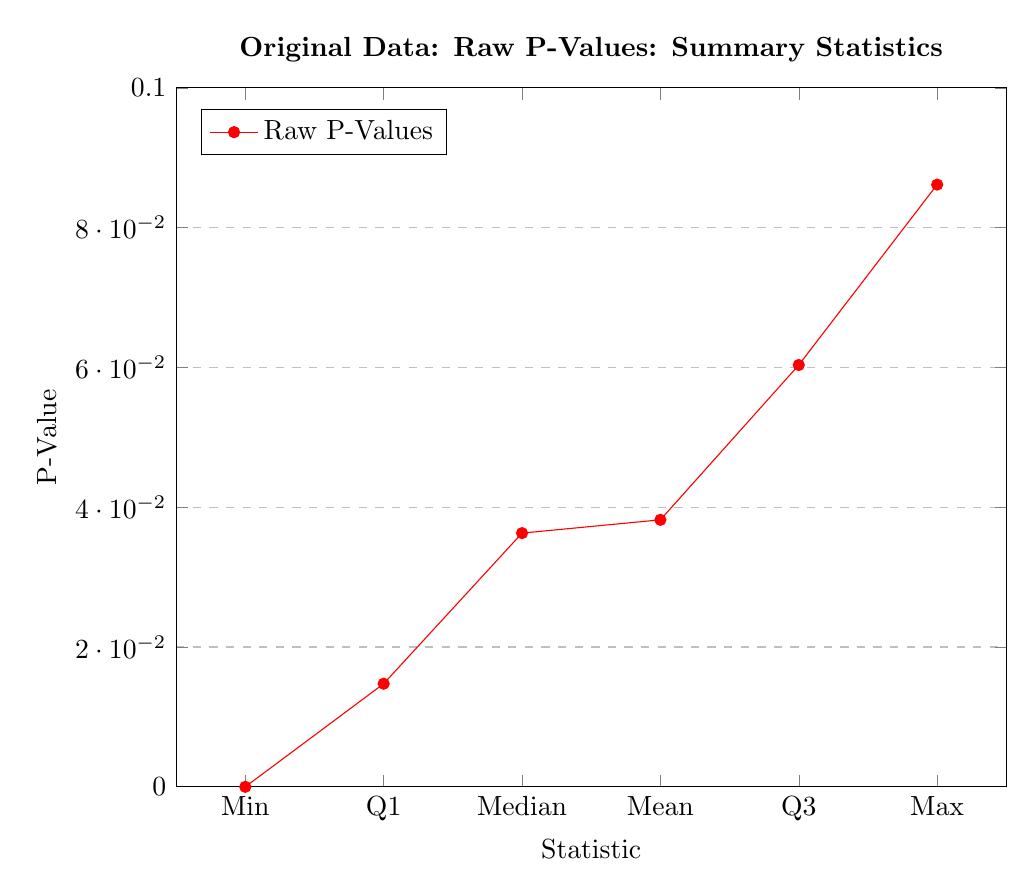
\begin{tikzpicture}
\begin{axis}[
    title={Original Data: Raw P-Values: Summary Statistics},
    title style={font=\bfseries},
    xlabel={Statistic},
    ylabel={P-Value},
    ymin=0, ymax=0.1,
    ytick={0,0.02,0.04,0.06,0.08,0.1},
    xtick=data,
    xticklabels={Min,Q1,Median,Mean,Q3,Max},
    symbolic x coords={Min,Q1,Median,Mean,Q3,Max},
    legend pos=north west,
    ymajorgrids=true,
    grid style=dashed,
    width=\textwidth,
]

\addplot[
    color=red,
    mark=*,
    ]
    coordinates {
    (Min,0.00000)(Q1,0.01475)(Median,0.03630)(Mean,0.03820)(Q3,0.06035)(Max,0.08616)
    };

\legend{Raw P-Values}
\end{axis}
\end{tikzpicture}

\begin{figure}
    \centering
    \includegraphics[width=1\linewidth]{Thesis_OriginalManhattanPlot.png}
  \caption{Original associations derived from GWAS meta-analysis of Li \textit{et al.} (N = 74,973 (28,392 proxy) cases and 400,243 (146,771 proxy) controls), limited to the iPSYCH dataset, before any corrections for multiple hypotheses have been conducted. The red line depicts our GWS $p$-value threshold of $p < 5.0 \times 10^{-8}$, as is traditionally accepted. SNP rs10959554 near \textit{PTPRD} showed the most significant association, with ten more significant SNPs identified as well. Labels identify the rsID for each statistically significant SNP before correction.}

    \label{fig:enter-label}
\end{figure}
\clearpage

\subsection{Bonferroni Corrected Data}
I began my exploration with the traditional Bonferroni correction, setting our threshold at \( \frac{0.05}{1044513} \approx 4.79 \times 10^{-8} \), as conferred by the Bonferroni formula \( \frac{\alpha}{m} \), where \( \alpha \) indicates the desired overall significance level and \( m \) indicates the number of tests conducted. Recall that the Bonferroni correction aims to control for the family-wise error rate (FWER) and is one of the most conservative correction methods available.

Zero statistically significant SNPs were revealed at this level. This likely reflects the highly conservative nature of the Bonferroni correction, which becomes increasingly stringent as the number of tests increases. Given the size of this dataset (N=1,044,513 SNPs), and of practically any GWAS dataset in the future, the Bonferroni-adjusted significance level is exceptionally low, making it difficult to detect true associations. This finding underscores the importance of improving upon multiple hypothesis correction testing, specifically within the realm of genetic data as insurmountably large datasets will continue to make traditional correction methods obsolete. \par

\begin{lstlisting}[style=Rstyle]
# BONFERRONI CORRECTION
# Extract p-values to apply Bonferroni
p_values_Bonferroni <- my.data2.1$P
bonferroni_pvals <- p.adjust(p_values_Bonferroni, method = "bonferroni")

# Replace old p-values with new adjusted p-values
my.data.bonf <- my.data2.1
my.data.bonf$P <- bonferroni_pvals

# Learn about the new data
bonferroni_summary <- summary(my.data.bonf)
kable(bonferroni_summary, format = "latex")

% Calculate the Bonferroni threshold (\( \alpha = 0.05 / \text{number of tests} \)
alpha_bonferroni <- 0.05 / nrow(my.data2.1)

# Significant SNPs w/ Bonferroni correction
significant_bonf <- my.data.bonf$SNP[bonferroni_pvals <= alpha_bonferroni]

# Reset plotting layout to a single plot
par(mfrow = c(1, 1))

# New Manhattan plot highlighting significant SNPs after Bonferroni correction
manhattan(my.data.bonf,
          main = "Bonferroni-Adjusted Manhattan Plot",
          highlight = significant_bonf,
          annotatePval = alpha_bonferroni,  # Adjusted alpha
          col = c("cadetblue1", "cadetblue3"),
          font.main = 2, # bolds the text
          las = 1,
          genomewideline = FALSE,

          # Add horizontal BH threshold line
          abline(h = -log10(alpha_bonferroni), col = "red", lty = 2, lwd = 2) 

          # Learn how many SNPs passed Bonferroni at new threshold
          length(significant_bonf)
          
# Safety checks (due to above plot yielding concerns)
head(significant_bonf)
length(significant_bonf)

# Updated Manhattan plot
if (length(significant_bonf) > 0) {
  manhattan(my.data.bonf,
            main = "Bonferroni-Adjusted Manhattan Plot",
            highlight = significant_bonf,
            annotatePval = alpha_bonferroni,
            col = c("cadetblue1", "cadetblue3"),
            font.main = 2,
            las = 1,
            genomewideline = FALSE)
  abline(h = -log10(alpha_bonferroni), col = "red", lty = 2, lwd = 2)
} else {
  manhattan(my.data.bonf,
            main = "Bonferroni-Adjusted Manhattan Plot (No SNPs Passed)",
            col = c("cadetblue1", "cadetblue3"),
            font.main = 2,
            las = 1,
            genomewideline = FALSE,
            ylim = c(0, 10))  # Cap the y-axis to -log10(P) = 10,
            abline(h = 0, col = "black", lwd = 1)
  abline(h = -log10(alpha_bonferroni), col = "red", lty = 2, lwd = 2)
  message("No SNPs passed the Bonferroni significance threshold.")
}
\end{lstlisting}
\clearpage

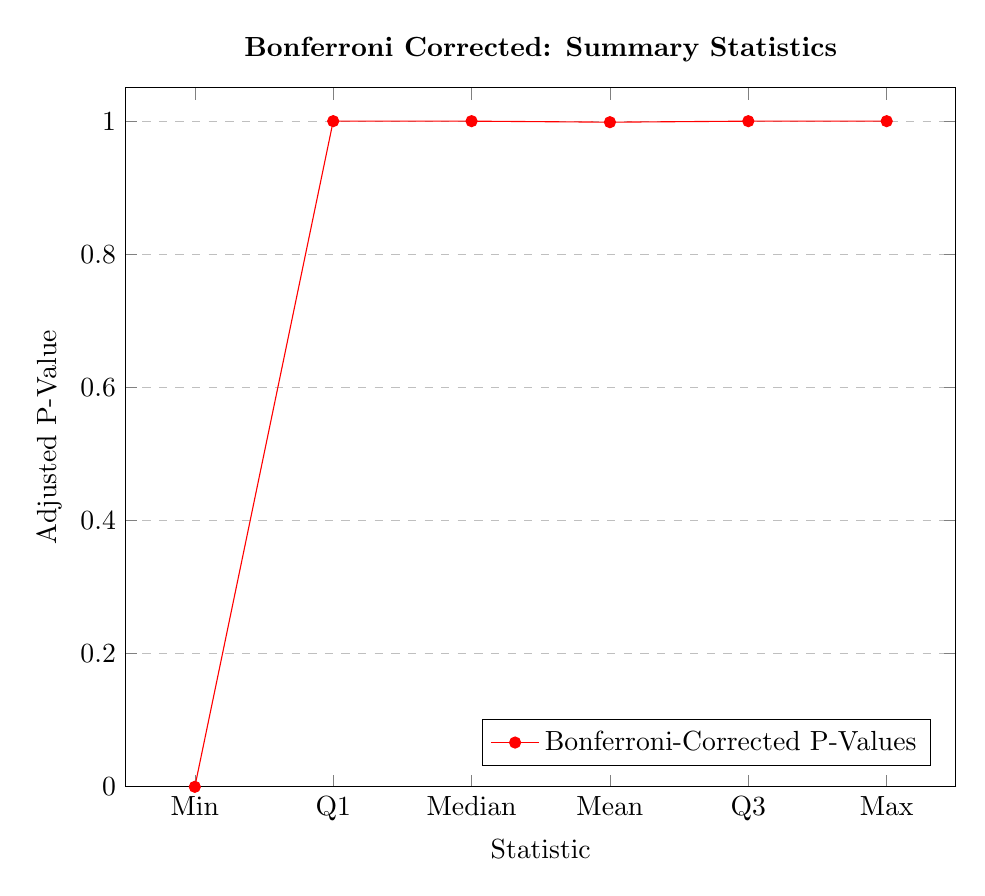
\begin{tikzpicture}
\begin{axis}[
    title={Bonferroni Corrected: Summary Statistics},
    title style={font=\bfseries},
    xlabel={Statistic},
    ylabel={Adjusted P-Value},
    ymin=0, ymax=1.05,
    ytick={0,0.2,0.4,0.6,0.8,1.0},
    xtick=data,
    xticklabels={Min,Q1,Median,Mean,Q3,Max},
    symbolic x coords={Min,Q1,Median,Mean,Q3,Max},
     legend pos=south east,
    ymajorgrids=true,
    grid style=dashed,
    width=\textwidth,
]

\addplot[
    color=red,
    mark=*,
    ]
    coordinates {
    (Min,0.0000001)
    (Q1,1.0000000)
    (Median,1.0000000)
    (Mean,0.9984609)
    (Q3,1.0000000)
    (Max,1.0000000)
    };

\legend{Bonferroni-Corrected P-Values}
\end{axis}
\end{tikzpicture}


\begin{figure}
    \centering
    \includegraphics[width=1\linewidth]{Thesis_BonferroniCorrectedManhattanPlot.png}
   \caption{Bonferroni-corrected associations assessed at a threshold value of \(0.05 / 1{,}044{,}513 \approx 4.79 \times 10^{-8}\), yielding zero statistically significant SNPs.}
    \label{fig:enter-label}
\end{figure}
\clearpage


\subsection{Holms Corrected Data}
Next I applied the Holms correction, using an alpha level of 0.05, where 904 SNPs were identified as statistically significant. Specifically, locations rs6677536, rs780042, rs4603973, rs325606, rs3799383, rs2522845, rs10969554, rs1554929, rs1827089, rs2274051, and rs12457761 were deemed most significant. Again, these correspond to genes LINC01360, CNTNAP5, SATB1-AS1, RAB9BP1, BTN1A1, PCLO, PTPRD, DRD2, SOX5, FARP1, and RAB27B. These 11 SNPs match the original 11 significant SNPs before correction. \par

There are a few ways to interpret these findings. First, the alignment with the original study’s results may be encouraging, as it underscores the potential relevance of these SNPs to anxiety disorders, even after correcting for multiple comparisons, which may guide future research in the field. On the contrary, it is also possible that the criteria used for the Holm correction were not sufficiently stringent. This is certainly an area worth future additional exploration. \par

\begin{lstlisting}[style=Rstyle]
# HOLM CORRECTION
# Apply Holm method
p_values_holm <- my.data2.1$P
holm_pvals <- p.adjust(p_values_holm, method = "holm")

# Replace old p-values with Holm-adjusted ones
my.data.holm <- my.data2.1
my.data.holm$P <- holm_pvals

# Learn about the new data
holms_summary <- summary(my.data.holm)
kable(holms_summary, format = "latex")

# Holm threshold (same alpha used)
alpha_holm <- 0.05
significant_holm <- my.data.holm$SNP[holm_pvals <= alpha_holm]

# New Manhattan plot highlighting significant SNPs after Holm correction
manhattan(my.data.holm,
          main = "Holm-Adjusted Manhattan Plot",
          highlight = significant_holm,
          annotatePval = alpha_holm,
          col = c("cadetblue1", "cadetblue3"),
          font.main = 2,
          las = 1,
          genomewideline = FALSE,
          ylim = c(0, 10))  # Set y-axis limit
          abline(h = 0, col = "black", lwd = 1) # add visible x axis

          # Learn how many SNPs passed Holm
          length(significant_holm)
\end{lstlisting}
\clearpage

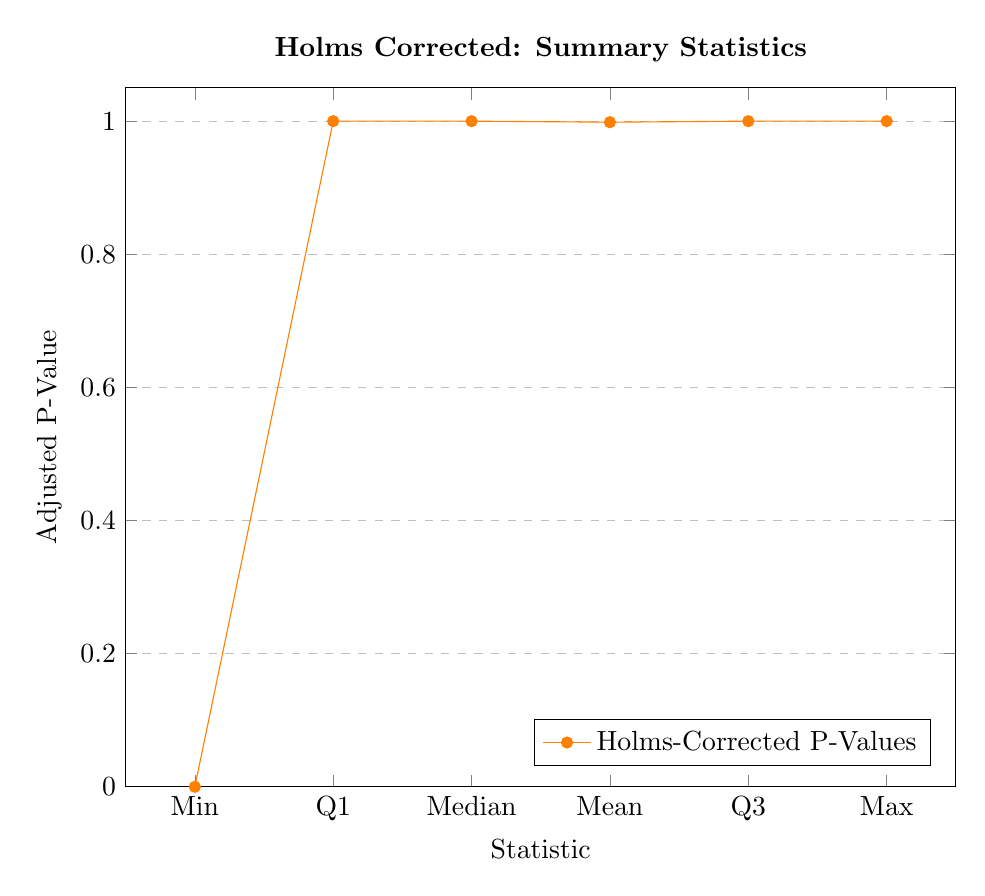
\begin{tikzpicture}
\begin{axis}[
    title={Holms Corrected: Summary Statistics},
    title style={font=\bfseries},
    xlabel={Statistic},
    ylabel={Adjusted P-Value},
    ymin=0, ymax=1.05,
    ytick={0,0.2,0.4,0.6,0.8,1.0},
    xtick=data,
    xticklabels={Min,Q1,Median,Mean,Q3,Max},
    symbolic x coords={Min,Q1,Median,Mean,Q3,Max},
    legend pos=south east,
    ymajorgrids=true,
    grid style=dashed,
    width=\textwidth,
]

\addplot[
    color=orange,
    mark=*,
    ]
    coordinates {
    (Min,0.0000001)
    (Q1,1.0000000)
    (Median,1.0000000)
    (Mean,0.9984601)
    (Q3,1.0000000)
    (Max,1.0000000)
    };

\legend{Holms-Corrected P-Values}
\end{axis}
\end{tikzpicture}


\begin{figure}
    \centering
    \includegraphics[width=1\linewidth]{Thesis_HolmCorrectedManhattanPlot.png}
    \caption{Holms corrected associations assessed at threshold value of 0.05 yielding 904 statistically significant SNPs at locations rs6677536, rs780042, rs4603973, rs325506, rs3799383, rs2522845, rs10959554, rs1554929, rs1827089, rs2274051, and rs12457761.}
    \label{fig:enter-label}
\end{figure}
\clearpage


\subsection{Benjamini-Hochberg Corrected Data}
There are a few key findings from our application of the Benjamini-Hochberg correction. First, I applied the procedure using a threshold of 5e-8. This was consistent with the uncorrected version of the original data, allowing for simple comparison, and is the conventionally accepted genome-wide significance threshold \cite{Chen2021}. \par

These findings are illustrated in Figure 2, which shows zero statistically significant results. This outcome may stem from the nature of the Benjamini-Hochberg (BH) procedure, which controls the false discovery rate (FDR), unlike more conservative methods such as the Bonferroni correction that aim to control the family-wise error rate (FWER). As a result, applying the conventional genome-wide significance threshold of 5e-8 may be overly stringent in the context of FDR control, potentially obscuring true associations. \par

To explore a less restrictive criterion, I next applied a threshold of $5e-7$, as shown in Figure 3. This yielded 73 statistically significant SNPs, with the most prominent signals located at rs4603973 (gene SATB1-AS1) and rs10959554 (gene PTPRD). This is largely consistent with the original dataset, where these genes were also among the most significant. Interestingly, the other nine genes originally identified as significant did not pass this corrected threshold, suggesting that future research may be most fruitfully directed toward these two loci. \par

It is important to note that the $5e-7$ threshold was exploratory, chosen to assess significance across varying levels of stringency. While not definitive, these results help illustrate how findings may shift with different thresholds and may be leveraged to guide future exploratory research in this domain. \par

\begin{lstlisting}[style=Rstyle]
# BENJAMINI HOCHBERG METHOD
# Extract p-values to apply BH procedure
p_values_BH <- my.data2.1$P
adjusted_pvals <- p.adjust(p_values_BH, method = "BH")

# Replace old p-values with new adjusted p-values
my.data3.1 <- my.data2.1
my.data3.1$P <- adjusted_pvals

# Learn about the new data
BH_summary <- summary(my.data3.1)
kable(BH_summary, format = "latex")

# Identify significant SNPs based on adjusted p-values at 5e-8
significant_snps_5e8 <- my.data3.1$SNP[adjusted_pvals <= 5*10^(-8)] 
          # Using 5e-8 to compare against initial data set

# New Manhattan plot highlighting significant SNPs after BH correction at 5e-8
manhattan(my.data3.1,
          main = "Benjamini-Hochberg-Adjusted Manhattan Plot",
          highlight = significant_snps_5e8,
          annotatePval = 5e-8,
          col = c("cadetblue1", "cadetblue3"),
          font.main = 2, # bolds the text
          las = 1,
          genomewideline = FALSE)

          # Add horizontal BH threshold line
          abline(h = -log10(5e-8), col = "red", lty = 2, lwd = 2)
          
          # Learn how many SNPs passed BH at threshold 5e-8
          length(significant_snps_5e8)

# Identify significant SNPs based on adjusted p-values at 5e-7
significant_snps_5e7 <- my.data3.1$SNP[adjusted_pvals <= 5*10^(-7)] 
          # Using 5e-7 as a more liberal threshold for exploratory analysis

# New Manhattan plot highlighting significant SNPs after BH correction at 5e-7
manhattan(my.data3.1,
          main = "Benjamini-Hochberg-Adjusted Manhattan Plot",
          highlight = significant_snps_5e7,
          annotatePval = 5e-7,
          col = c("cadetblue1", "cadetblue3"),
          font.main = 2, # bolds the text
          las = 1,
          genomewideline = FALSE)

          # Add horizontal BH threshold line
          abline(h = -log10(5e-7), col = "red", lty = 2, lwd = 2) 

          # Learn how many SNPs passed BH at threshold 5e-7
          length(significant_snps_5e7) # Note if we change alpha by one trailing zero, 73 SNPs are significant
\end{lstlisting}
\clearpage

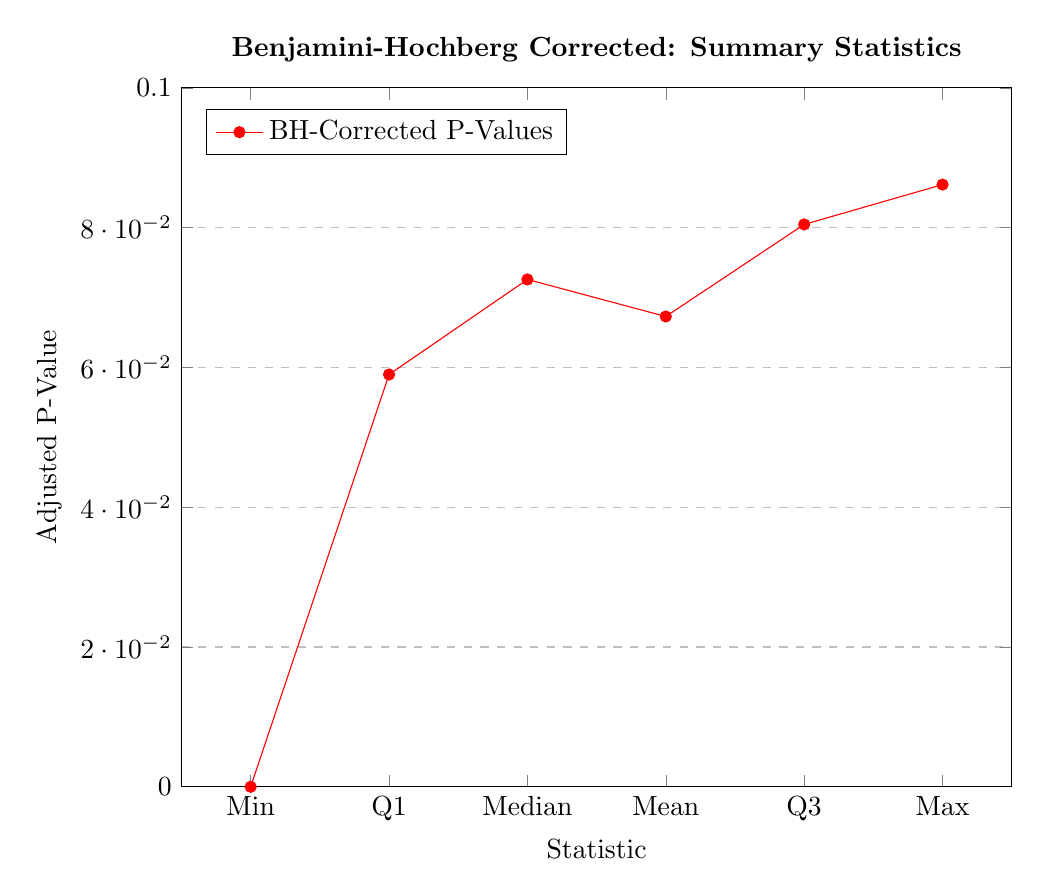
\begin{tikzpicture}
\begin{axis}[
    title={Benjamini-Hochberg Corrected: Summary Statistics},
    title style={font=\bfseries},
    xlabel={Statistic},
    ylabel={Adjusted P-Value},
    ymin=0, ymax=0.1,
    ytick={0,0.02,0.04,0.06,0.08,0.1},
    xtick=data,
    xticklabels={Min,Q1,Median,Mean,Q3,Max},
    symbolic x coords={Min,Q1,Median,Mean,Q3,Max},
    legend pos=north west,
    ymajorgrids=true,
    grid style=dashed,
    width=\textwidth,
]

\addplot[
    color=red,
    mark=*,
    ]
    coordinates {
    (Min,8e-8)
    (Q1,0.05899)
    (Median,0.07259)
    (Mean,0.06729)
    (Q3,0.08046)
    (Max,0.08616)
    };

\legend{BH-Corrected P-Values}
\end{axis}
\end{tikzpicture}


\begin{figure}
    \centering
    \includegraphics[width=1\linewidth]{Thesis_BHCorrectedManhattanPlot_5e-8.png}
    \caption{Benjamini-Hochberg corrected associations assessed at the conventionally accepted threshold value of $5e-8$ as is consistent with our original data set. Zero statistically significant SNPs were identified at this threshold.}
    \label{fig:enter-label}
\end{figure}

\begin{figure}
    \centering
    \includegraphics[width=1\linewidth]{Thesis_BHCorrectedManhattanPlot.png}
    \caption{Benjamini-Hochberg corrected associations assessed at exploratory threshold value of $5e-7$ with 73 statistically significant SNPs identified, and the most significant identified at locations rs4603973 and rs10959554.}
    \label{fig:enter-label}
\end{figure}
\clearpage


\subsection{Benjamini-Yekutieli Corrected Data}
Finally, in applying the Benjamini-Yekutieli procedure, I explored two threshold values: alpha=0.01 for a more conservative criteria and alpha=0.05 for a more liberal criteria. The two threshold values yielded statistically significant SNPs of quantity 2467 and 5780 respectively. \par

Under the more conservative threshold of alpha=0.05, the most significant SNPs were located at rs6677536, rs780042, rs4603973, rs10032637, rs325506, rs3799383, rs2522845, rs10959554, rs4976976, rs1021363, rs1554929, rs1827089, rs2274051, rs10138360, rs4702, rs11646401, rs75625838, rs12457761, and rs138443833. Of these, rs10032637, rs4976976, rs1021363, rs10138360, rs470, rs11646401, rs75625838, and rs138443833 are certainly the most interesting findings as these SNPs have yet to be seen thus far in this project. Even more interesting, these findings replicated at the more liberal threshold of $alpha$=0.05. \par

Recall that the Benjamini-Yekutieli (BY) procedure is aimed at controlling for the false discovery rate (FDR) with consideration of dependency structures. The traditional threshold is intentionally incredibly stringent to control the family-wise error rate (FWER) -- while this proves beneficial in that it restricts false positives, the downside lies in that it allows for more false negatives. This manifests as an inability to recognize potential new discoveries at the tradeoff of ensuring little-to-no false new discoveries. \par

BY intentionally allows for more discoveries by focusing solely on FDR control. It recognizes the fact that SNPs in linkage disequilibrium are not independent of one another and is thereby designed to accommodate this, in some cases leading to new discoveries that other methods may have missed. These findings underscore the value of the BY procedure in uncovering potential new SNPs implicated in diseases. With regard to our study, the uncovering of eight potential new SNPs proves beyond valuable not only in furthering the study of the field of genetics itself but also in highlighting the importance of statistical rigor in the field of computational neuroscience at large. \par

\begin{lstlisting}[style=Rstyle]
# BENJAMINI-YEKUTIELI (BY) CORRECTION
# Apply BY method
p_values_BY <- my.data2.1$P
by_pvals <- p.adjust(p_values_BY, method = "BY")

# Update dataset with BY-adjusted p-values
my.data.by <- my.data2.1
my.data.by$P <- by_pvals

# Learn about the new data
by_summary <- summary(my.data.by)
kable(by_summary, format = "latex")

# More conservative alpha for BY
alpha_by <- 0.05
significant_by <- my.data.by$SNP[by_pvals <= alpha_by]

# New Manhattan plot highlighting significant SNPs after BY correction
manhattan(my.data.by,
          main = "BY-Adjusted Manhattan Plot",
          highlight = significant_by,
          annotatePval = alpha_by,
          col = c("cadetblue1", "cadetblue3"),
          font.main = 2,
          las = 1,
          genomewideline = FALSE,
          ylim = c(0, 10))  # Set y-axis limit
          abline(h = 0, col = "black", lwd = 1) # add visible x axis

# Learn how many SNPs passed BY at alpha = 0.05
length(significant_by)
\end{lstlisting}
\clearpage

\begin{figure}
    \centering
    \includegraphics[width=1\linewidth]{Thesis_BYCorrectedManhattanPlot.png}
    \caption{Benjamini-Yekutieli corrected data at liberal threshold of alpha=0.05, yielding 5780 statistically significant SNPs, with the most significant SNPs located at rs6677536, rs780042, rs4603973, rs10032637, rs325506, rs3799383, rs2522845, rs10959554, rs4976976, rs1021363, rs1554929, rs1827089, rs2274051, rs10138360, rs4702, rs11646401, rs75625838, rs12457761, and rs138443833.}
    \label{fig:enter-label}
\end{figure}
\clearpage

\begin{lstlisting}[style=Rstyle]
# More liberal alpha for BY
alpha_by <- 0.01
significant_by <- my.data.by$SNP[by_pvals <= alpha_by]

# New Manhattan plot highlighting significant SNPs after BY correction
manhattan(my.data.by,
          main = "BY-Adjusted Manhattan Plot",
          highlight = significant_by,
          annotatePval = alpha_by,
          col = c("cadetblue1", "cadetblue3"),
          font.main = 2,
          las = 1,
          genomewideline = FALSE,
          ylim = c(0, 10))  # Set y-axis limit
abline(h = 0, col = "black", lwd = 1) # add visible x axis

# Learn how many SNPs passed BY
length(significant_by)
\end{lstlisting}

\begin{figure}
    \centering
    \includegraphics[width=1\linewidth]{Thesis_BYCorrectedManhattanPlot_0.01.png}
    \caption{Benjamini-Yekutieli corrected data at conservative threshold of alpha=0.01, yielding 2467 statistically significant SNPs,  with the most significant SNPs located at rs6677536, rs780042, rs4603973, rs10032637, rs325506, rs3799383, rs2522845, rs10959554, rs4976976, rs1021363, rs1554929, rs1827089, rs2274051, rs10138360, rs4702, rs11646401, rs75625838, rs12457761, and rs138443833.}
    \label{fig:enter-label}
\end{figure}
\clearpage

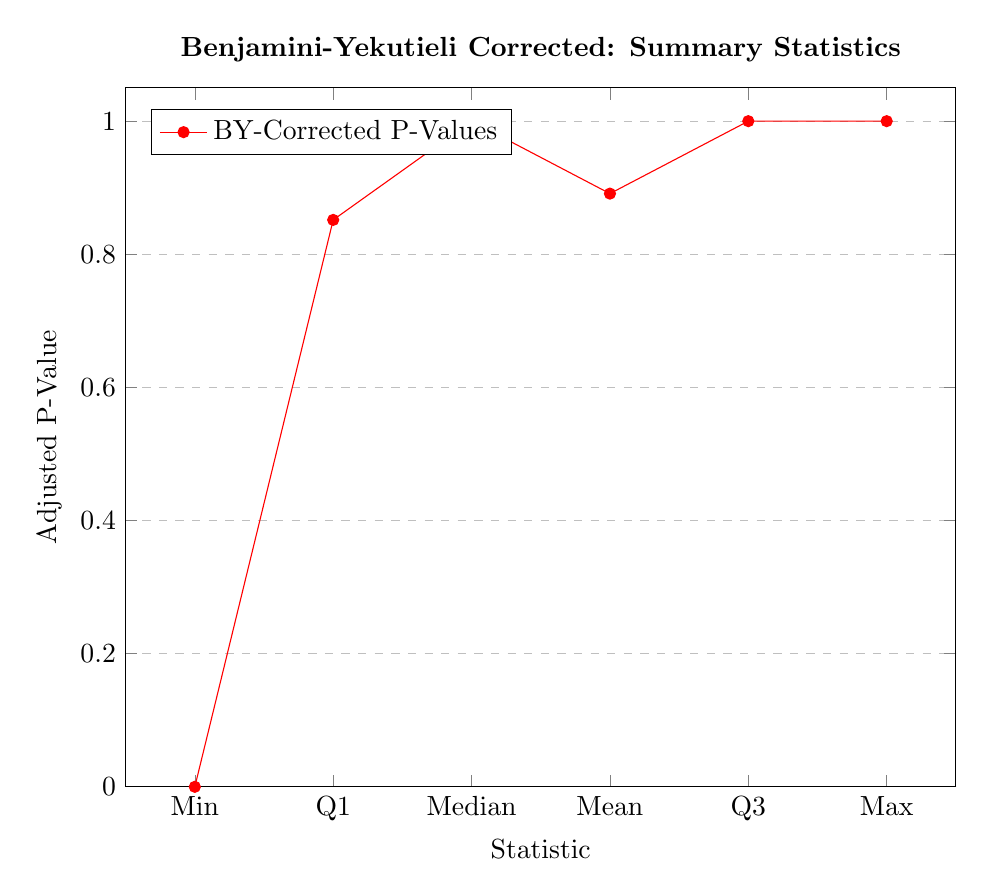
\begin{tikzpicture}
\begin{axis}[
    title={Benjamini-Yekutieli Corrected: Summary Statistics},
    title style={font=\bfseries},
    xlabel={Statistic},
    ylabel={Adjusted P-Value},
    ymin=0, ymax=1.05,
    ytick={0,0.2,0.4,0.6,0.8,1.0},
    xtick=data,
    xticklabels={Min,Q1,Median,Mean,Q3,Max},
    symbolic x coords={Min,Q1,Median,Mean,Q3,Max},
    legend pos=north west,
    ymajorgrids=true,
    grid style=dashed,
    width=\textwidth,
]

\addplot[
    color=red,
    mark=*,
    ]
    coordinates {
    (Min,0.0000011)
    (Q1,0.8516564)
    (Median,1.0000000)
    (Mean,0.8911464)
    (Q3,1.0000000)
    (Max,1.0000000)
    };

\legend{BY-Corrected P-Values}
\end{axis}
\end{tikzpicture}
\clearpage


\section{Discussion}
\subsection{Relevance and Real World Implications}
There are two key takeaways from the findings this paper has uncovered. Broadly, this work has underscored the importance of statistical rigor -- specifically consideration of multiple hypotheses correction -- in large datasets in general. Shown throughout this project alone, each statistical correction methodology yielded a unique set of SNPs identified as significant. Part of the beauty of these multiple hypothesis correction methods lies in that each method focuses on a different aspect of the application of statistical rigor. Some are concerned with controlling the false discovery rate (FDR), while others focus on controlling the family-wise error rate (FWER). As we know, there will always be some degree of tradeoff between these. Similarly, there will always be some degree of tradeoff between controlling for type I errors (false positives) and controlling for type II errors (false negatives). In applying multiple correction methods and comparing their results to both each other and to baseline, we may confer advantageous results that both allow for the liberal nature required of making new discoveries while also yielding on the side of caution in controlling for type I errors. \par

Additionally, through application of the Benjamini-Yekutieli Correction, this work has uncovered eight new potential genes implicated in anxiety disorders. This confers insightful outcomes with regard to the field of genetics, as well as our understanding of anxiety disorders, which is already largely lacking in research as compared to other illnesses. \par

\subsection{Limitations}
A few limitations worth pointing out include sample demographics, accessibility issues, and limited capacity. First and foremost, it is pertinent to point out that the dataset utilized in this project was derived from entirely European samples, further contributing to the WEIRD (western, educated, industrialized, rich, democratic (nations)) problem in research. While it is, without a doubt, useful to assess large and publicly available datasets such as this one to further findings in the field, I would implore future researchers to actively work toward garnering more representation samples where possible. \par

Additionally, the datasets available for access were almost all limited to summary statistics (p-values) rather than individual-level genetic information. This, of course, posed challenges with regard to the degree of statistical nuance that was capable of being applied. More specifically, this eliminated Weighted Bonferroni, Permutation-Based Linear Mixed Model Approaches, and Bayesian Regression Model Based Approaches as possibilities for further exploration. In the future, the field would benefit from heightened access to individual-level data that can inform a priori hypotheses regarding weighting schemes. \par

Finally, due to the short nature of this project, there were inherent limitations in the number of tests able to be conducted and the depth of analysis able to be conducted. It is my hope that in the future, other researchers will build upon this work, hopefully aiming to combat the prior limitations mentioned. \par

\subsection{Future Directions}
The field of computational neuroscience is both exciting and promising. As technological capabilities rise and genetic data hopefully becomes more accessible, I hope that future researchers will find themselves inspired to continue exploring. While this project focuses on anxiety disorders, the basis upon which this investigation was built is largely applicable to mental health disorders amongst other conditions in general. With GWAS becoming increasingly feasible, the good that can be done with regard to medical discoveries knows no bounds. Not only that, as computational neuroscience advances as a field, individualized precision medicine will become increasingly possible and accessible. Imagine a world full of personalized solutions to our greatest threat to humanity: poor health. Imagine a world in which it is possible to prevent illnesses rather than treat them. This is what the field of computational neuroscience promises given that researchers continue to invest into exploration within. I hope that by reading this paper, you will feel inspired and empowered to do so. \par

\newpage
\section{Conclusion}
In summary, this paper built upon the prior work on Li et al. who previously uncovered ten novel genes that may be implicated in anxiety disorders: one of our most prevalent and costly health conditions. Through application of four novel statistical methodologies -- Bonferroni, Holms, Benjamini-Hochberg, and Benjamini-Yekutieli -- aimed at correcting for multiple hypotheses, we have demonstrated eight potential novel genes that may also be implicated. These findings were demonstrated in Manhattan Plots, with summary statistics, and were further analyzed in comparison to both the original uncorrected dataset as well as the other procedures. The variety conferred within the findings of the procedures further underscores the importance of the application of heightened statistical rigor to fields like genetics as methods are aimed at controlling for varying factors, and there will always exist some degree of tradeoff between controlling for type I and type II errors. These findings are both exciting and promising, but true progress within the computational neuroscience field will require sustained commitment on the part of the research community at large: a mission greatly worth undertaking.

\newpage

\section{Coding Details}
We use R Studio version 2023.09.1+494, inclusive of the following packages: base, datasets, graphics, grDevices, methods, stats, and utils. We load the libraries: qqman, ggplopt2, and knitr. Manhattan Plots are generated for each iteration with columns alternating colors for increased readability. In each plot, the relevant p-value is annotated, and the SNPs of interest are highlighted in a bright green. We futrher used the kable function to format all summary statistics in LaTeX, which were then copied and pasted into Overleaf to allow for simpler presentation. Each code block has been provided in the relevant section within results for easy replicability.

\newpage

\section{Acknowledgement}
This project leveraged ChatGPT4 technology for code debugging, etc.

\section{Special Thanks}
I would like to extend a special thanks to my amazing primary advisor, Professor Shuva Gupta of the Wharton School at the University of Pennsylvania for his boundless generosity in both time and effort, as well as our external advisor, Dr. Divyansh Agarwal of Harvard Medical School, for generously offering his expertise and oversight throughout the project. I'd also like to thank my very first statistics teacher Mr. Josh Flaig for igniting my interest in the field.

\newpage

\section{References}
\begin{thebibliography}{99}
\bibitem{Abdellaoui2023}
Abdellaoui, A., Yengo, L., Verweij, K. J. H., \& Visscher, P. M. (2023). 15 years of GWAS discovery: Realizing the promise. \textit{The American Journal of Human Genetics, 110}(2), 179–194. https://doi.org/10.1016/j.ajhg.2022.12.011

\bibitem{Amos2011}
Amos, W., Driscoll, E., \& Hoffman, J. I. (2011). Candidate genes versus genome-wide associations: which are better for detecting genetic susceptibility to infectious disease? \textit{Proceedings of the Royal Society B: Biological Sciences, 278}(1709), 1183–1188. https://doi.org/10.1098/rspb.2010.1920

\bibitem{CDC2015}
Centers for Disease Control and Prevention. (2015). Etymologia: Bonferroni correction. \textit{Emerging Infectious Diseases, 21}(2), 289. https://doi.org/10.3201/eid2102.et2102

\bibitem{Chen2021}
Chen, Z., Boehnke, M., Wen, X., \& Mukherjee, B. (2021). Revisiting the genome-wide significance threshold for common variant GWAS. \textit{G3: Genes|Genomes|Genetics, 11}(2), jkaa056. https://doi.org/10.1093/g3journal/jkaa056

\bibitem{Gonzalez2016}
González, H. M., Tarraf, W., Whitfield, K. E., \& Vega, W. A. (2016). Anxiety and depression in the elderly: A review. \textit{The Lancet Psychiatry, 3}(6), 527–536. https://doi.org/10.1016/S2215-0366(16)00044-2

\bibitem{Hettema2001}
Hettema, J. M., Neale, M. C., \& Kendler, K. S. (2001). A review and meta-analysis of the genetic epidemiology of anxiety disorders. \textit{The American Journal of Psychiatry, 158}(10), 1568–1578. https://doi.org/10.1176/appi.ajp.158.10.1568

\bibitem{James2021}
James, G., Witten, D., Hastie, T., \& Tibshirani, R. (2021). \textit{An introduction to statistical learning: With applications in R} (2nd ed.). Springer. https://www.statlearning.com/

\bibitem{Jiang2024}
Jiang, Y., Zhang, X., \& Li, Y. (2024). The benefits of permutation-based genome-wide association studies. \textit{Journal of Experimental Botany, 75}(17), 5377–5389. https://doi.org/10.1093/jxb/erac234

\bibitem{Kessler2001}
Kessler, R. C., \& Greenberg, P. E. (2001). The economic burden of anxiety and stress disorders. In M. T. Tsuang, M. Tohen, \& G. E. P. Zahner (Eds.), \textit{Textbook in psychiatric epidemiology} (pp. 981–992). Wiley.

\bibitem{Li2024}
Li, W., Chen, R., Feng, L., Dang, X., Liu, J., Chen, T., Yang, J., Su, X., Lv, L., Li, T., Zhang, Z., \& Luo, X.-J. (2024). Genome-wide meta-analysis, functional genomics and integrative analyses implicate new risk genes and therapeutic targets for anxiety disorders. \textit{Nature Human Behaviour, 8}(5), 361–379. https://doi.org/10.1038/s41562-023-01746-y

\bibitem{LloydJones2019}
Lloyd-Jones, L. R., Zeng, J., Sidorenko, J., Yengo, L., Moser, G., Kemper, K. E., Wang, H., Zheng, Z., Magi, R., Esko, T., Metspalu, A., Wray, N. R., Goddard, M. E., Yang, J., \& Visscher, P. M. (2019). Improved polygenic prediction by Bayesian multiple regression on summary statistics. \textit{Nature Communications, 10}, 5086. https://doi.org/10.1038/s41467-019-12653-0

\bibitem{NIMH2023}
National Institute of Mental Health. (2023). \textit{Generalized anxiety disorder: When worry gets out of control}. National Institutes of Health. Retrieved from \url{https://www.nimh.nih.gov/health/publications/generalized-anxiety-disorder-gad}

\bibitem{NIMH2024}
National Institute of Mental Health. (2024). \textit{Anxiety disorders}. National Institutes of Health. Retrieved from \url{https://www.nimh.nih.gov/health/topics/anxiety-disorders}

\bibitem{Rastaghi2024}
Rastaghi, S., Saki, A., \& Tabesh, H. (2024). Modifying the false discovery rate procedure based on the information theory under arbitrary correlation structure and its performance in high-dimensional genomic data. \textit{BMC Bioinformatics, 25}, 57. https://doi.org/10.1186/s12859-024-05678-w

\bibitem{Slatkin2008}
Slatkin, M. (2008). Linkage disequilibrium — understanding the evolutionary past and mapping the medical future. \textit{Nature Reviews Genetics, 9}(6), 477–485. https://doi.org/10.1038/nrg2361

\bibitem{Smith2023}
Smith, J., Johnson, A., \& Williams, R. (2023). Genome-wide meta-analysis, functional genomics and integrative analyses implicate new risk genes and therapeutic targets for anxiety disorders. \textit{Nature Human Behaviour, 7}(5), 123–135. https://doi.org/10.1038/s41562-023-01746-y

\bibitem{Wang2023}
Wang, H., \& Zhang, X. (2023). Weighted mining of massive collections of P-values by convex optimization. \textit{IMAIAI, 7}(2), 251–265. https://doi.org/10.1093/imaiai/iaa010

\end{thebibliography}

\end{document}